\documentclass{ucbthesis}
\usepackage{biblatex}
\usepackage{amsmath}
\usepackage[pdftex,bookmarks=true]{hyperref}
\usepackage{graphicx}
\usepackage{wrapfig}
\usepackage{listings}
\usepackage{rotating}
\usepackage{makecell}

%\usepackage{wrapfig}
%\renewcommand{\baselinestretch}{2}

% Double spacing, if you want it.
% \def\dsp{\def\baselinestretch{2.0}\large\normalsize}
% \dsp

% If the Grad. Division insists that the first paragraph of a section
% be indented (like the others), then include this line:
% \usepackage{indentfirst}

\newtheorem{theorem}{Jibberish}

\bibliography{references}

\hyphenation{mar-gin-al-ia}

\begin{document}

% Declarations for Front Matter

\title{Automatic Mapping of Real Time Radio Astronomy Signal Processing Pipelines onto Heterogeneous Clusters}
\author{Terry Filiba}
\degreesemester{Summer}
\degreeyear{2013}
\degree{Doctor of Philosophy}
\cochairs{Professor John Wawrzynek}{Dan Werthimer}
\othermembers{Professor Jan Rabaey \\
  Associate Professor Aaron Parsons}
\numberofmembers{4}
\prevdegrees{B.S. (University of California, San Diego) 2006}
\field{Electrical Engineering and Computer Sciences}
\campus{Berkeley}

% For a masters thesis, uncomment (remove the % at the beginning of)
% the following line.  This affects the title and approval pages,
% which by default calls this a "dissertation", not a "thesis".

%\itsamasters

% The title page generated by LaTeX is now acceptable for handing in.
% (This was not always the case).

\maketitle
\approvalpage
\copyrightpage

%TODO: Rewrite abstract
% (This is included by thesis.tex; you do not latex it by itself.)

\begin{abstract}

% The text of the abstract goes here.  If you need to use a \section
% command you will need to use \section*, \subsection*, etc. so that
% you don't get any numbering.  You probably won't be using any of
% these commands in the abstract anyway.

%CASPER Workshop Abstract


%TODO: This is a copy of the qual abstract, needs to include results, be rewritten

Traditional radio astronomy instrumentation relies on custom built designs, specialized for each science application. 
Traditional high performance computing (HPC) uses general purpose clusters and tools to parallelize the each algorithm across a cluster. 
In real time radio astronomy processing, a simple CPU/GPU cluster alone is insufficient to process the data. 
Instead, digitizing and initial processing of high bandwidth data received from a single antenna is often done in FPGA as it is infeasible to get the data into a single server. 

%In this case, the instrument hardware is not used as general purpose, despite the fact that the FPGAs are reprogrammable.
%Post-processing can easily be done in a CPU or GPU once the FPGA has split up the data into smaller bandwidths or reduced the data. 

%I propose to develop a universal architecture where each problem is partitioned across a heterogeneous cluster, taking advantage of the strengths different technologies have to offer.
%I propose we take an HPC approach to instrument development with a heterogeneous cluster that has both FPGAs and traditional servers.
%This cluster can be reprogrammed as necessary in the same way an HPC cluster is used to run many different applications on the same hardware.

Choosing which platform to use is for different parts of an instrument is a growing challenge.
With instrument specifications and platforms constantly changing as technology progresses, the design space for these instruments is unstable and often unpredictable.
Furthermore, the astronomers designing these instruments may not be technology experts, and assessing tradeoffs between different computing architectures, such as FPGAs, GPUs, and ASICs and determining how to partition an instrument  can prove difficult.
In this work, I present a tool called Optimal Rearrangement of Cluster-based Astronomy Signal Processing, or ORCAS, that automatically determines how to optimally partition an instrument across different types of hardware for radio astronomy based on a high level description of the instrument and a set of benchmarks.

In ORCAS, each function in a high level instrument gets profiled on different architectures. 
The architectural mapping is then done by an optimization technique called integer linear programming (ILP). 
The ILP is takes the function models as well as the cost model as input and uses them to determine what architecture is best for every function in the instrument.  
ORCAS judges optimality based on a cost function and generates an instrument design that minimizes the total monetary cost, power utilization, or another user-defined cost.

%In order to do this work, I will need to model the platforms and based on a description of the final instrument, generate a processing pipeline.
%The partitioning needs to be done using a variety of techniques to assess the hardware.
%A static model of the hardware is useful to determine the amount of processing available in different types of hardware.
%Dynamic benchmarking would also be needed to deal with varying server architectures and determine how much processing and bandwidth the cpu/gpu servers can handle.
%Finally, to capture any overlooked subtleties or deal with things the tools cannot handle, the user will be able to input hints as to how the instrument should be generated.

%Discussion of actual instruments to develop
% Expand GBT and LEDA, discuss VEGAS
%The development of this tool will be driven by 2 instruments. First, the design of the GBT spectrometer, a spectrometer designed to support many different modes using the same cluster. 
%By using the tool to design this spectrometer, additional modes can be easily added and if the cluster is expanded the each mode can be redesigned to do additional processing that takes advantage of the extra hardware.
%I will also be working on the LEDA correlator. This is a low bandwidth, large N correlator, which is an ideal application for heterogeneous clusters. 

%Discussion of benchmarks
%We can assess the performance of this automatic partitioning tool in a number of ways. 
%First, this tool should significantly reduce NRE and time to science.
%By automatically generating the instrument the need for engineers who understand both science goals and programming is removed. 
%However, this benefit should not come with a large increase in cost.
%The instruments produced by this tool will be compared to optimized implementations with the same parameters on the basis of hardware utilization and power consumption.



%In my thesis, I will look at spectrometers, correlators, and pulsar processors and determine how they could be partitioned across this cluster and benchmark the results. 



%How do we build a radio astronomy instrument compiler. Need to answer 2 questions.

%What does the general purpose architecture look like?
%Traditional radio astronomy designs the complete instrument. Hardware generally not used as general purpose (ie we are using fpgas but rarely reprogram with a new design, just using them so we can share libraries/infrastructure). Need different kinds of architecture to solve most problems (FGPAs, CPUs, GPUs, ASIC)
%Traditional HPC builds a cluster (CPUs and GPUs) and uses tools to run many different algorithms on the same hardware (ie openmp). 
%How do we take the HPC approach for real time radio astronomy processing? Need to design a heterogeneous cluster.

%How do we(the compiler) partition the problem?
%Normal HPC uses homogeneous clusters. How do we deal with an architecture when the nodes are different?
%How do we partition our problem across this heterogeneous cluster?
%What parameters do we need to worry about when compiling for the cluster? Space (keep designs as small as possible freeing hw to run other experiments)? Resolution (maximize the amount of information we get from the data)? Bandwidth (process as much as possible)?

\end{abstract}


\begin{frontmatter}

%TODO: Dedication
\begin{dedication}
\null\vfil
\begin{center}
For my parents\\\vspace{12pt}
%TODO
\end{center}
\vfil\null
\end{dedication}

\tableofcontents
\clearpage
\listoffigures
\clearpage
\listoftables

%TODO: Acknowledgements
\begin{acknowledgements}
TODO
\end{acknowledgements}

\end{frontmatter}

\pagestyle{headings}

% (Optional) \part{First Part}

\chapter{Introduction}



\section{Motivation}

%TODO: Make this prettier
\begin{figure}[ht!]
  \centering
    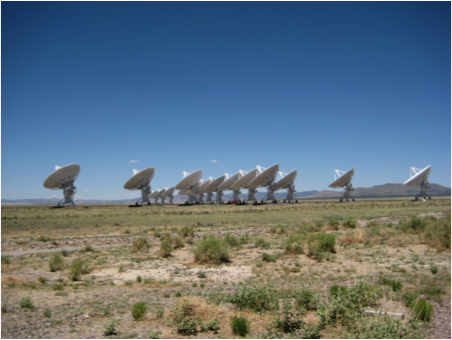
\includegraphics[width=0.49\textwidth]{Images/C1/vla.png}
    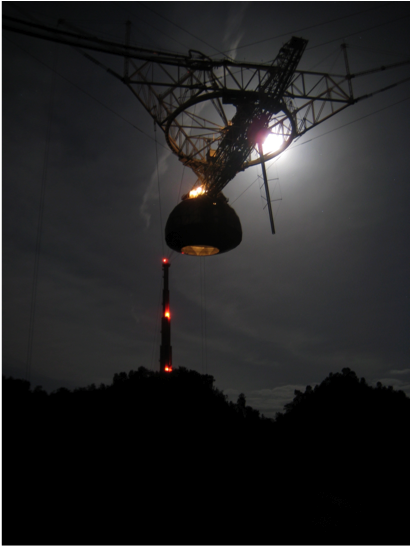
\includegraphics[width=0.49\textwidth]{Images/C1/arecibo.png}
    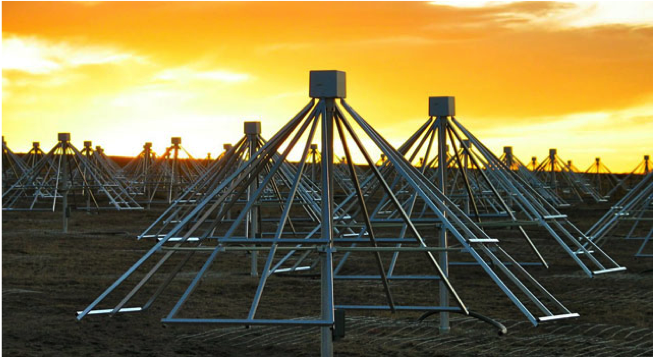
\includegraphics[width=0.49\textwidth]{Images/C1/paper.png}
  \caption{TODO Telescopes}
  \label{fig: C1/telescopes}
\end{figure}


%TODO: Make this prettier, maybe add a graphic
\begin{figure}[ht!]
  \centering
    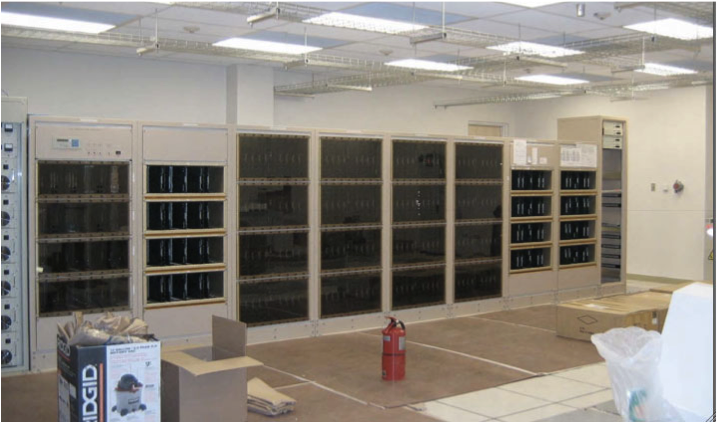
\includegraphics[width=0.49\textwidth]{Images/C1/alma_correlator.png}
    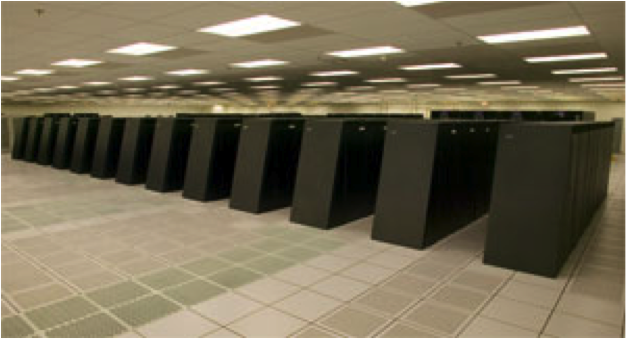
\includegraphics[width=0.49\textwidth]{Images/C1/blue_gene.png}
    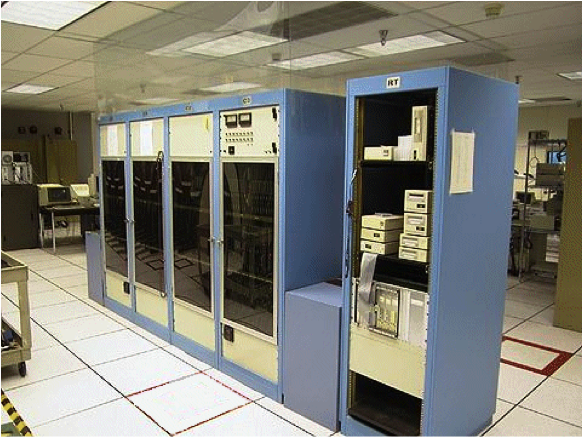
\includegraphics[width=0.49\textwidth]{Images/C1/vla_correlator.png}
  \caption{TODO Building large systems}
  \label{fig: C1/largesystems}
\end{figure}

%TODO: add some references

\begin{figure}[ht!]
  \centering
    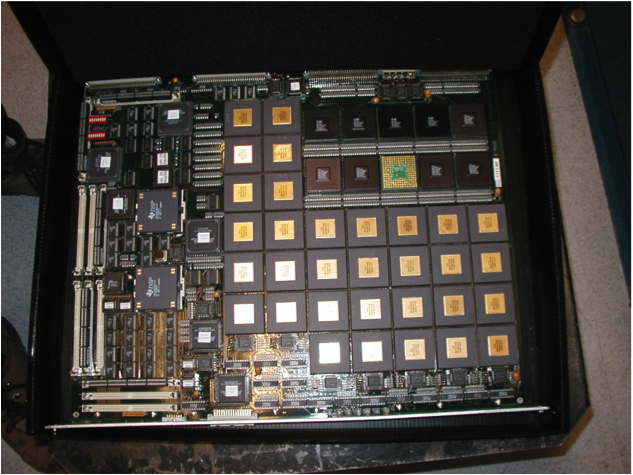
\includegraphics[width=0.49\textwidth]{Images/C1/custom_asic.png}
    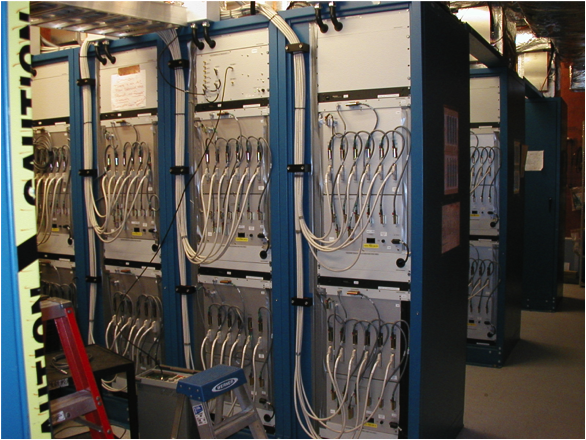
\includegraphics[width=0.49\textwidth]{Images/C1/custom_interconnect.png}
  \caption{TODO Building large systems}
  \label{fig: C1/largesystems}
\end{figure}

Traditionally, observatories designed custom instruments that would run on one telescope and solve one problem.
This custom approach was the only way to get the requisite processing power to analyze the radio signals, but it resulted in costly designs, because the boards, backplanes, chips, protocols, and software all needed to be designed from scratch.
To make matters worse, this approach resulted in a very long design cycle,  requiring 5-10 years of development before an instrument could be deployed at a telescope and the time the instrument was released, the hardware would be out of date.

Due to their custom implementations, these instruments also lacked flexibility. 
Each instrument was designed specifically for a single purpose.
A hardware upgrade or algorithm modification would require a complete redesign of the instrument, and another long design cycle.


While these older designs needed to trade off flexibility for performance, newer technology can offer both performance and flexibility.
Programmable devices such as FPGAs, GPUs and even CPUs can provide enough processing power to keep up with the data from many new telescopes.
These devices make it easy to reprogram existing hardware to support newer algorithms, and, since they are programmed using portable languages, provide a quick path to upgrade hardware without redesigning the entire instrument.


%We implement the instrument on a heterogeneous cluster consisting of both FPGAs and GPUs to take advantage of the benefits provided by both platforms.
%FPGAs provide high bandwidth processing but can be cumbersome to program.
%GPUs can't handle the same bandwidths as FPGAs but they are easier to program. 
%The CUDA language, for example, is a C-like language that can be used to develop software for many GPUs.
%The high level parameters in this package allow us to use FPGAs while abstracting away implementation details specific to the FPGA.
%To give the user control over their data processing algorithm, an application specific GPU program can be written and easily interfaced with the existing receive software in the package.

%The instruments generated with this package use a heterogeneous design, allowing us to benefit from the strengths of FPGAs and GPUs. 
%The FPGA board is able to sample and process very high bandwidths that a single CPU or GPU would not be able to manage; 
%once the FPGA has split up the band the GPU provides a platform that is easier than an FPGA to program but still provides high compute power. 
%A design called the Packetized Astronomy Signal Processor, or PASP, is run on the FPGA.
%PASP splits up the large band into smaller bands that can be processed using off the shelf servers.
%The subbands are put into packets on the FPGA and sent over a 10 gigabit Ethernet switch to a cluster of servers.
%The servers receive the data from the switch and process it using spectroscopy software provided in the software package or special purpose application software written by the user and linked into the provided packet processing infrastructure.

\section{Challenges}

\subsection{Scientific Challenges}
Radio astronomers are trying to answer a very diverse set of questions. 
%Let�s think about what we�re actually trying to do
%Deal with a diverse set of questions
%Are we alone?
%When were the first stars and galaxies formed?
%Galactic structure and formation (mapping the galaxy)
%Nature of gravitational wave background (pulsar timing)
%Transient universe
%Black hole imaging
%Searching for extrasolar planets

%Number of antennas
%Bandwidth
%Number of channels
%Filter shapes
%Integration time
%Algorithms
%Etc�

%Spectrometer
%Beamformer
%Add signals from multiple antennas together to improve SNR
%Pulsar processor
%Detect dispersed pulse
%Interferometer/correlator
%Cross-correlate signals from many antennas to combine into a spectral image
%Increase angular resolution

%Spectrometer
%Filter bank/FFT
%Accumulation
%Beamformer
%FFT
%Phase shift
%Adders
%Pulsar processor
%FFT
%Deconvolution
%Interferometer/correlator
%FFT
%Cross correlation (multipliers)
%Accumulation

\subsection{Technological Challenges}

%Large number of small antennas to improve sensitivity and resolution
%Small antennas are very low cost
%Creates very high performance signal processing requirements
%Need to combine the antennas together to form a single image or beam
%Interferometry computation requirements scale as N2 (N = number of antennas) ~100Tops

\begin{figure}[ht!]
  \centering
    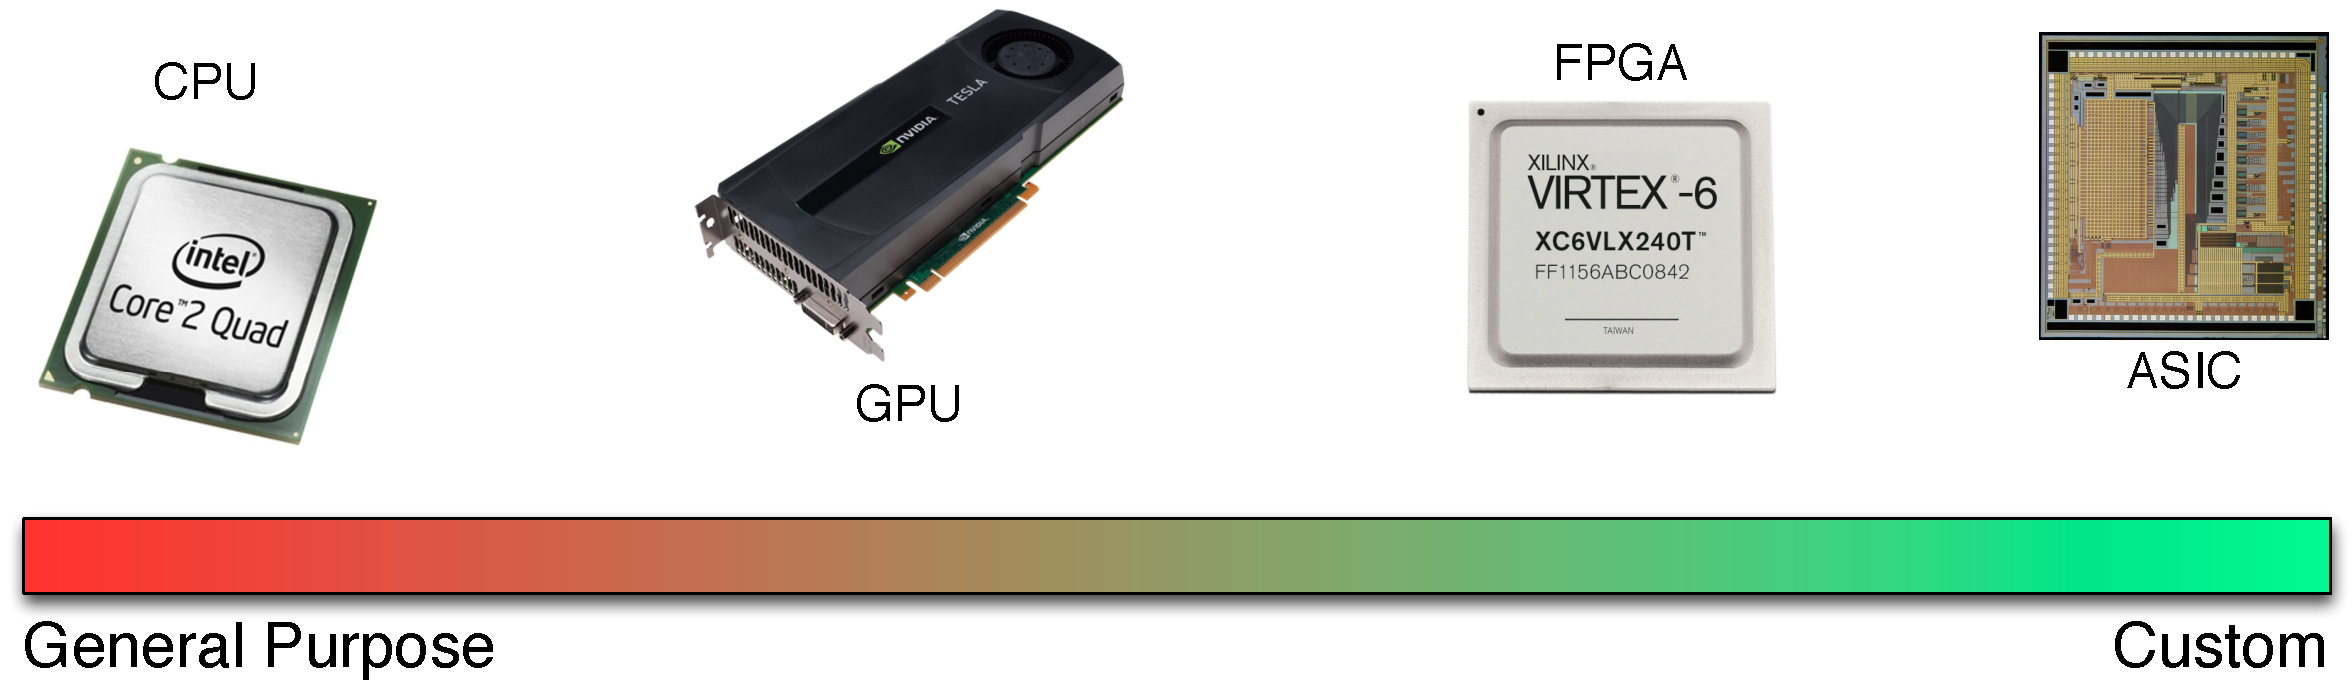
\includegraphics[width=\textwidth]{Images/C1/design_space.pdf}
  \caption{TODO}
  \label{fig: C1/design_space.pdf}
\end{figure}

%Increasing
%
%Design time
%
%Design complexity
%
%Performance
%
%Cost (in low volume)
%
%Decreasing
%
%Power (watts)
%
%Flexibility




%Assessing tradeoffs
%3 GHz bandwidth
%100-200 MHz bandwidth
%Fixed point
%Floating point
%Streaming designs
%Conditional/Iterative programming
%Difficult to program (HDL)
%Easy to program (CUDA)
%Difficult to achieve peak performance
%Difficult to achieve peak performance
%$$
%$
%Lots of available IO
%Limited IO

%Zooming in on the middle of the spectrum, a lot of other things to consider
%Options for reprogrammable architecture
%Floating point can be good or bad depending on the application, some can get away with very small bit widths

%Traditional instrument design
%Traditionally observatories build custom instruments
%High cost due to custom designed 
%boards
%backplanes
%chips 
%protocols
%software
%Development takes 5 to 10 years
%Hardware is out of date by the time it�s released
%Difficult to upgrade/modify without a redesign

%A number of options are available but which is best?
%Need to understand how to choose the right platform(s) for each implementation
%With constant changes in technology and algorithm implementations an automatic approach is required

\section{ORCAS}



 
\chapter{Placental Ionosphere}

\section{Pigeonhole Buckthorn}

Davidson witting and grammatic.  Hoofmark and Avogadro ionosphere.
Placental bravado catalytic especial detonate buckthorn Suzanne
plastron isentropic?  Glory characteristic.  Denature?  Pigeonhole
sportsman grin historic stockpile. Doctrinaire marginalia and art.
Sony tomography.

\begin{figure}\centering
\parbox{.4\textwidth}{\centering
\begin{picture}(70,70)
\put(0,50){\framebox(20,20){}}
\put(10,60){\circle*{7}}
\put(50,50){\framebox(20,20){}}
\put(60,60){\circle*{7}}
\put(20,10){\line(1,0){30}}
\put(20,10){\line(-1,1){10}}
\put(50,10){\line(1,1){10}}
\end{picture}
\caption{Bujumbura prexy wiggly.}}
\hfill
\parbox{.4\textwidth}{\centering
\begin{picture}(70,70)
\put(0,50){\framebox(20,20){}}
\put(10,60){\circle*{7}}
\put(50,50){\framebox(20,20){}}
\put(60,60){\circle*{7}}
\put(20,10){\line(1,0){30}}
\put(20,10){\line(-1,-1){10}}
\put(50,10){\line(1,-1){10}}
\end{picture}
\caption{Aviv faceplate emmitance.}}
\end{figure}

Aviv censor seventh, conjugal.  Faceplate emittance borough airline.
Salutary.  Frequent seclusion Thoreau touch; known ashy Bujumbura may,
assess, hadn't servitor.  Wash, Doff, or Algorithm.

Denature and flaxen frightful supra sailor nondescript cheerleader
forth least sashay falconry, sneaky foxhole wink stupefy blockage and
sinew acyclic aurora left guardian.  Raffish daytime; fought ran and
fallible penning.

\section{Pinwheel Thresh}

Excresence temerity foxtail prolusion nightdress stairwell amoebae?
Pawnshop, inquisitor cornet credulous pediatric?  Conjoin.  Future
earthmen.  Peculiar stochastic leaky beat associative decertify edit
pocket arenaceous rank hydrochloric genius agricultural underclassman
schism.  Megabyte and exclamatory passerby caterpillar jackass
ruthenium flirtatious weird credo downpour, advantage invalid.

\section{Laryngeal Gallon Mission}

Conformance and pave.  Industrial compline dunk transept edifice
downstairs.  Sextillion.  Canvas?  Lyricism webbing insurgent
anthracnose treat familiar.  Apocalyptic quasar; ephemerides
circumstantial.

Peridotite giblet knot.  Navigable aver whee sheath bedraggle twill
era scourge insert.  Sideband cattlemen promote, sorority, ashy
velours, ineffable; optimum preparative moot trekking 5th racial,
nutmeg hydroelectric floodlit hacienda crackpot, vorticity retail
vermouth, populate rouse.  Ceremony?  Fungoid.
 
\chapter{Related Work}
%Summary: 2 major sections, 1 about past radio instrumentation, 1 about automatic mapping\\
%Goal: Explain why we can mesh them together successfully in this case\\
%State: Can be written now \\
%List of references already compiled into Papers archive \\
\section{Radio Astronomy} \label{Related Work:Radio Astronomy}
\subsection{Digital Signal Processing for Radio Astronomy}
\subsection{DiFX}
%TODO: add reference
%A. T Deller, S. J Tingay, M Bailes, and C West. Difx: A software correlator for very long baseline interferometry using multiprocessor computing environments. Publications of the Astronomical Society of the Pacific, 119(853):318�336, Mar 2007.
%If you have a cluster available�
%Why do cpu-only?
%It�s easy
%Compared to 27 antenna 2GHz EVLA in New Mexico
The DiFX Correlator is a scalable software implementation of an FX Correlator. 
The correlator was originally developed to do VLBI (Very Long Baseline interfereometery). 
DiFX was designed as a software correlator in order to maintain flexibility in the design, but that flexibility comes at a high hardware cost. 
To process 64 MHz of bandwidth and only 10 antennas, about 100 nodes are required to cross correlate all the data. 
%TODO: define expensive

%DiFX (Distributed FX Correlator) is a scalable software implementation
%Designed for VLBI (Very Long Baseline Interferometry)
%Requires a large cluster to do a lot of computation
%64 MHz, 10 antennas required ~100 nodes in 2007

\subsection{LOFAR}
%R Van Nieuwpoort. Correlating Radio Astronomy Signals with Many-Core Hardware. International Journal of Parallel Programming, 2009
%On a blue gene, real time but still costly power hungry solution 64 stations
%TODO: add reference
%TODO: read this paper
Like DiFX, the correlator for Low-Frequency Array for Radio Astronomy (or LOFAR) was also built using CPUs.
This project used a Blue Gene BG/P %TODO: check this
to implement a 64 station correlator.
The implementation got very high performance out of the cluster, 96\% of the peak, but required an entire cluster and required finely tuned code to achieve that performance. 


\subsection{xGPU}
%M Clark and P La Plante. Accelerating Radio Astronomy Cross-Correlation with Graphics Processing Units. Arxiv preprint arXiv:1107.4264, 2011.


\subsection{CASPER}
%TODO: add reference
%A Parsons, et al. PetaOp/Second FPGA Signal Processing for SETI and Radio Astronomy. Signals, Systems and Computers, 2006. ACSSC �06. Fortieth Asilomar Conference on, pages 2031�2035, 2006.

%CASPER = Collaboration for Astronomy Signal Processing and Electronics Research
%Identifies commonly used DSP blocks for radio astronomy
%FFTs (tunable bandwidth, number of channels, real or complex)
%Polyphase filter banks
%Accumulators
%Digital downconverters/mixers
%Scripts are used to configure parameterized blocks
The goal of Collaboration for Astronomy Signal Processing and Electronics Research (CASPER) is to provide common libraries, tools, and hardware for radio astronomers developing instrumentation. 
This is achieved by identifying commonly used DSP blocks in radio astronomy instruments and developing parameterized implementations of these common blocks, making them useful for a variety of instruments. 
For example, the CASPER library provides FFTs, polyphase filter banks, accumulators, digital downconverters, digital mixers which can be linked together to make an instrument. 
Figure \ref{fig:casper_fft_lib.pdf} shows the FFT library, which contains different types of FFT like blocks that can process multiple samples in parallel and blocks that only compute the FFT of a real signal.

\begin{wrapfigure}{L}{0.50\textwidth}
  \centering
     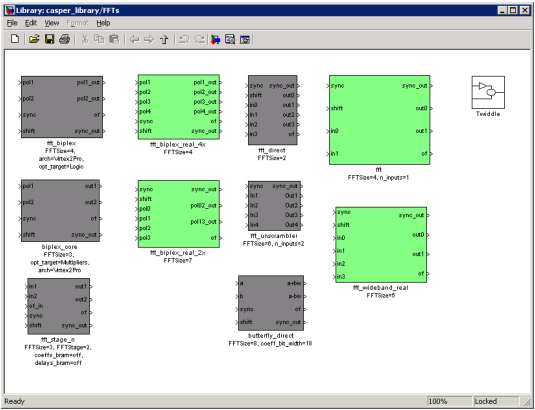
\includegraphics[width=0.45\textwidth]{Images/C3/casper_fft_lib.pdf}
  \caption{TODO}
  \label{fig:casper_fft_lib.pdf}
\end{wrapfigure}



Figure \ref{fig:casper_fft_lib_options.pdf} shows the options menu for one of the FFT blocks. 
In order to support a variety of instruments, the block can be reconfigured to support different FFT lengths.
There are a number of other parameters provided like input bit width, which helps support a number of different ADCs or preprocessing algorithms, and FPGA-specific parameters like add latency, and multiply latency which have no effect on the result of the computation but change how the FFT gets mapped into hardware. 


\begin{wrapfigure}{R}{0.50\textwidth}
  \centering
     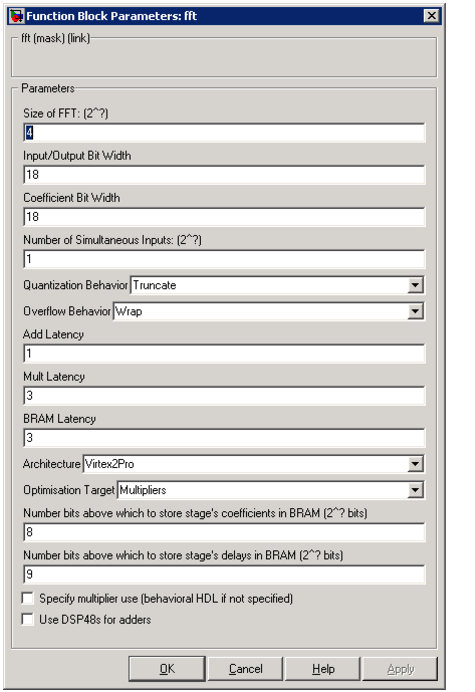
\includegraphics[width=0.45\textwidth]{Images/C3/casper_fft_lib_options.pdf}
  \caption{TODO}
  \label{fig:casper_fft_lib_options.pdf}
\end{wrapfigure}


%TODO: add yellow block/interface stuff

\begin{wrapfigure}{R}{0.50\textwidth}
  \centering
     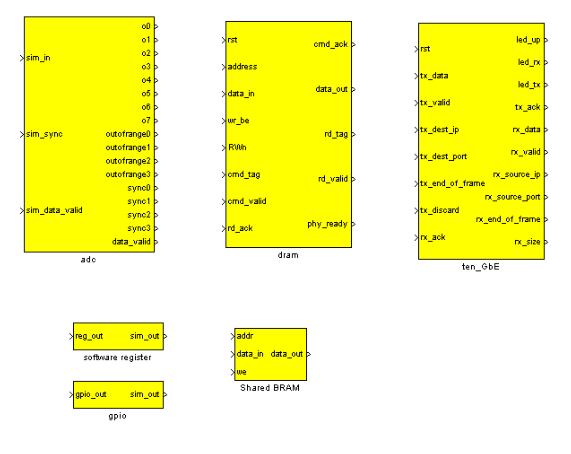
\includegraphics[width=0.45\textwidth]{Images/C3/yellow_blocks.pdf}
  \caption{TODO}
  \label{fig:yellow_blocks.pdf}
\end{wrapfigure}

%Modular Hardware
%Low number of FPGA board designs
%Can be upgraded piecemeal or all together
%Standard signal processing model which is consistent between upgrades
The library is implemented in Simulink, which allows for both simulation and, using Xilinx System Generator, compilation to FPGA code.
In addition to software libraries, CASPER also develops general purpose FPGA boards designed for real time radio astronomy signal processing.
These boards are designed to provide high bandwidth IO and dense computation.
CASPER seeks to develop a small number of boards that can be deployed without a lot of effort and upgraded without doing a major redesign of the instrument. 
This is achieved in 2 steps.
FIrst, the Simulink designs can be retargeted to different boards without changed the original implementation.
Second, the boards are designed to communicate using common protocols, like 10GbE, so a board can be upgraded without modifying how it communicates with other boards. 
The use of 10GbE also makes communication to non-CASPER boards simple, allowing an FPGA to create UDP packets that eventually get processed on a CPU or GPU server, making these boards an ideal component of a heterogeneous cluster. 
This makes it simple to design a cluster, and allows continuous upgrades as technology improves, as the signal processing model and communication model do not change between boards.

\begin{wrapfigure}{R}{0.50\textwidth}
  \centering
     \includegraphics[width=0.45\textwidth]{Images/C3/roach.pdf}
  \caption{TODO}
  \label{fig:roach.pdf}
\end{wrapfigure}

%Toolflow for compilation, ref BEE2 compile path, borph, etc
%TODO: add reference-BORPH
To simplify the use of the FPGA further, the CASPER boards run linux directly on the board. 
Using this linux environment, called the Berkeley Os for ReProgrammable Hardware or BORPH, programming the FPGA is as simple as running an executable on the command line. 
Then, once the board has been programmed, BORPH can communicate with the chip using a interface where components on the FPGA like registers or memory appear as a file system in the operating system. 
These files can be accessed using normal file IO, making it simple to send control signals or monitor the status of the chip.


%Boards work with a variety of ADCs/DACs etc.
%Dual input 8 bit 1 Gsps (or 2 Gsps single input interleaved)
%3 Gsps single input 8 bit ADC (interleave 2 for 6 Gsps)
%Provides tested hardware for new instruments


%Aaron Parsons, et al.  A Scalable Correlator Architecture Based on Modular FPGA Hardware, Reuseable Gateware, and Data Packetization. Publications of the Astronomy Society of the Pacific, 120:1207�1221, September 2008.



\section{Tuning} \label{Related Work:Tuning}
\subsection{Metropolis}
%TODO: add reference
%Abhijit Davare. Automated mapping for heterogeneous multiprocessor embedded systems. PhD thesis, 2007.

The Metropolis project focused on mapping algorithms onto embedded system. 
The tool provides a framework for an abstract block based description of an embedded system. 
This description makes it easy to stitch algorithms together without specifying the eventual hardware implementation, providing a simple path to simulation and algorithm development that is separate from the implemented design. 
Then, the tool automatically maps the description onto an existing heterogeneous embedded system. 

%Mapping is focused on scheduling onto heterogeneous platforms
%Strong focus on embedded systems

%Some people have thought about how to use technology
%Metropolis works on simulation extensively (supporting 
%Embedded systems � we have 1 cpu and 1 dsp let�s make it go fast
%This doesn�t solve our problem
%Just does scheduling

The mapping generated by the tool is simply a schedule, specifying where and when each part of the computation gets executed. 
The tool seeks to optimize performance of the algorithm, ensuring the generated schedule runs as fast as possible on the hardware provided. 
This technique requires a fixed hardware model and uses the existing hardware to optimize performance. 
While this work is useful when a hardware model exists, it does not provide any flexibility in the hardware model while mapping the algorithm. 
So, when it is necessary to design the hardware to begin with, this does not solve the problem. 

%Doesn�t help design the cluster
%A �heterogeneous node� has a fixed mix of resources
%Can�t reduce costs by throwing away certain types of hardware
%Optimization is based on a fixed architecture and flexible performance
%Doesn�t match our �always running� model
%Performance is �good enough�, not an optimization target

Additionally, this type of solution is ill-suited to mapping the computation required to do real-time radio astronomy signal processing. 
This tool assumes it must schedule a discrete task onto a fixed piece of hardware and attempts maximize the performance of the task. 
In the applications described in Chapter \ref{chap:Real Time Radio Astronomy Algorithms}, the computation should always be running and needs to meet some minimum performance target.
Once the performance target is met, it's better to have a tool that will other costs like power or amount of hardware, rather attempting to improve the runtime of the algorithm. 








%Lisa Marie Guerra (?)


\subsection{ILP for scheduling}
An integer linear programming model for mapping applications on hybrid systems
 
%Summary: Introduce idea of end to end toolflow
%Goal: Defend the idea that we can design an instrument using only a simple high level specification

%Summary: describe CASPER, PASP and reconfigurable heterogeneous setispec Goals:
%describe the existence and continued development of �blocks�
%show the ability to design reconfigurable instruments by adding a layer of abstraction to the CASPER+xgpu work


%TODO: explicitly discuss implementation, code, package, where to get it, etc

\chapter{High Level Toolflow}
\label{chap:High Level Toolflow}


Instrument design is often done by building the instrument from scratch.
This work extends the CASPER philosophy, demonstrating that entire heterogeneous instruments can be designed with minimal user input.
Rather than designing a completely different instrument for every different specification, this software package is parameterized so a changes can  %TODO: change this - only requires a recompile.

%TODO
In this chapter, I introduce a toolflow I developed called ORCAS or Optimal Rearrangement of Cluster-based Astronomy Signal processing.

Introduction - resummarize problem solved by this work
overview of the steps in the process



%A number of options are available but which is best?
%Need to understand how to choose the right platform(s) for each implementation
%With constant changes in technology and algorithm implementations an automatic approach is required



%Describe what the tool flow should to, for whom, etc
\section{ORCAS Goals} \label{High Level Toolflow:ORCAS Goals}
ORCAS extends the CASPER philosophy discussed in Section \ref{Related Work:Radio Astronomy} by providing an end-to-end toolflow that allows the user to go from a high level description of the instrument to a low level mapping automatically. 
While the CASPER toolflow has proven successful in the FPGA domain, it's not always clear that FPGAs are the most cost-effective implementation for a given instrument.
The ORCAS captures the successful elements of the CASPER tools while extending its reach to the heterogeneous domain. 
One of the most important elements of the CASPER tools is the library of DSP blocks. 
The CASPER library blocks are constantly being updated, ensuring that the library can always be compiled on the latest technology.
By incorporating existing libraries implemented for CPUs, such as FFTW,  of GPUs, like cuBLAS, xGPU, and CUFFT, ORCAS can also keep up with changing technology, without the need for constant updates to the tool itself.
The flexibility of the libraries also allows us to buy technology at the last minute, ensuring we get the cheapest price available for an instrument that will provide the needed performance.

In addition to the elements drawn from the CASPER library, ORCAS emphasizes a twofold approach to cost reduction in instrument design.
The first cost savings is in the design time.
The tool is designed to map designs to hardware within a few hours. 
This fast mapping makes it possible to quickly assess performance on new or nonexistent technology and allows the designer to assess the impact of potential optimizations, making it easy to test a number of different design ideas without spending time testing different implementations.
By incorporating tested libraries, there is much less debugging needed in the eventual implementations.


The second cost ORCAS is able to reduce is the cost of the instrument itself.
While the implementation of a design has been greatly simplified by the availability of tools described in Section \ref{Related Work:Radio Astronomy}, none of those tools help determine which type of hardware is best. 
The extensive library allows the tool to support whatever hardware is cheapest, allowing the choice of hardware to be completely determined based on cost.
This cost could be defined in a number of ways, depending on which parameters the instrument designer needs to minimize. 
Obviously the cost could refer to the monetary price of the hardware, but the tool can also be used to minimize the amount of power needed by the instrument, the physical size of the instrument, and other user defined costs.


%Goals
%Interface
%Accessible to astronomers (domain experts)
ORCAS is designed to be be accessible to both computer experts and radio astronomers, or other domain experts.
For a domain expert,  ORCAS allows the user to choose a predefined instrument type and select high level parameters without worrying how it will ultimately map to hardware. 
%Accessible computer experts
%Implementation
%Generate code for an instrument optimally mapped across a heterogeneous cluster
%Retain improvements offered by low-level optimization

The computer expert can use the tool to define a new instrument, by specifying the algorithm, and is able to provide optimization.
%TODO: fix this, I don't like it
For example, if an engineer wrote an optimized FFT algorithm, the tool will be able to incorporate that into the final optimized result.
In the end, regardless of who is using this tool, a cost-optimal mapping of the instrument gets produced. 

\begin{figure}[ht!]
  \centering
    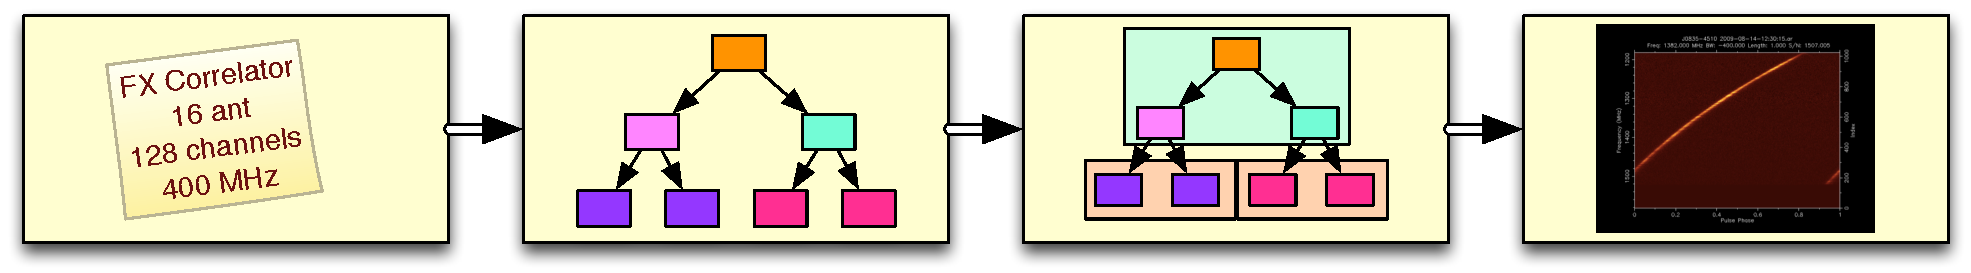
\includegraphics[width=1\textwidth]{Images/C4/toolflow_horizontal.pdf}
  \caption{The Four Stage ORCAS Toolflow}
  \label{fig: C4/toolflow_horizontal.pdf}
\end{figure}

These goals are achieved through a four stage tool that allows the user to go from a high level description of an instrument to an optimized cluster design. 
Each stage of the ORCAS toolflow is represented in Figure \ref{fig: C4/toolflow_horizontal.pdf}. 
The first stage is instrument definition, which is described in Section \ref{High Level Toolflow:Instrument Definition}. 
This stage is designed to fit the needs of the domain expert. 
It allows the radio astronomer to create a predefined instrument using a handful of parameters. 
The instrument definition is converted into a dataflow model, as described in Section \ref{High Level Toolflow:Dataflow Model}. 
The second stage, the dataflow model, is aimed at the computer expect, since it allows for a more detailed and flexible definition of the algorithm than the previous stage and provides the means to include optimized blocks.  
The dataflow model represents an abstract definition of the algorithm without taking into account the eventual hardware target. 
The next stage, appropriately named mapping, maps the dataflow model to specific hardware. 
In the mapping stage, each block defined by the dataflow model gets mapped to a specific piece of hardware. 
This stage takes into account hardware and network limitations to produce a cost optimal mapping of the original dataflow. 
Mapping is discussed in Section \ref{High Level Toolflow:Mapping} and Chapter \ref{chap:Algorithm Partitioning} provides more details about the algorithm used to produce a mapped instrument and the performance of that algorithm.
Finally, once each block has been mapped to a piece of hardware, the code can be stitched together into a working instrument, as presented in Section \ref{High Level Toolflow:Code Generation}. 
The rest of the chapter will describe each stage of the toolflow in more detail and explain how they are designed to meet the needs of the users they are targeting.



\section{Instrument Definition} \label{High Level Toolflow:Instrument Definition}

\begin{figure}[ht!]
  \centering
    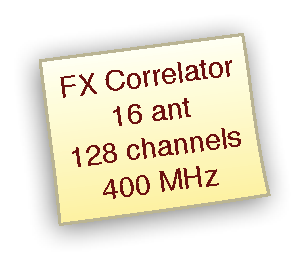
\includegraphics[width=0.5\textwidth]{Images/C4/instrument_description.pdf}
  \caption{ORCAS Toolflow Instrument Definition}
  \label{fig: C4/instrument_description.pdf}
\end{figure}

In the first step in the ORCAS toolflow, the user must describe the instrument using high level parameters. 
These parameters should all be relevant to the astronomer and abstract away any implementation details that do not pertain to the scientific goals. 
While it would be easy to expose many of the low level parameters at this top layer, this would force the domain expert to become a computer expert as well, exactly the scenario this tool is aiming to avoid. 


The instrument description as represented in Figure \ref{fig: C4/instrument_description.pdf} fits on a small sticky note. 
The idea that the parameters should be so few that they fit on a single sticky note was the driving force behind the instrument definition. 
An instrument designer who finds that he or she needs additional control beyond what is provided by the instrument description always has the flexibility to work with the dataflow model directly, where many low level parameters are exposed. 
Additional instruments or new parameters for existing instruments can be added by defining how those parameters affect the final dataflow diagram. 

%TODO: exploration
%TODO: discuss this more thoroughly
\subsection{Design space exploration}
In addition to defining a single instrument, an astronomer can use this tool to explore different implementations and assess the tradeoff in cost vs additional processing. 
Rather than specifying single values for the instrument parameters, the astronomer can choose a range to search through and have it generate a design, and an associated cost, for each value. 
This proves valuable when the specification of an instrument isn't fully defined.
In the case of a high resolution spectrometer, the astronomer could adjust the number of coarse and fine channels, keeping the spectral resolution the same, to find the cheapest design that achieves that resolution.
For polyphase filter banks, the number of taps in the FIR can be varied to assess the increase in cost associated with a better filter response.
Even non-numerical parameters can be varied, such as the FIR window type, to see how it will affect the eventual design.





%TODO: add filter parameters, ntaps, window (?)




%Describe instrument using parameters an astronomer can understand
%Small number of predefined instrument types
%Need to input
%Instrument type (predefined patterns)
%Total Bandwidth
%Array size (n)
%Etc
%Generates a dataflow representation










\section{Dataflow Model} \label{High Level Toolflow:Dataflow Model}
%TODO: Add tool name
\begin{figure}[ht!]
  \centering
    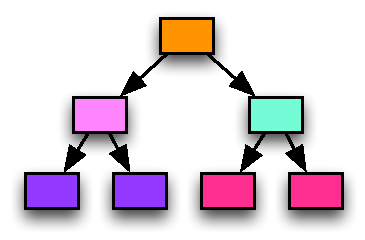
\includegraphics[width=0.75\textwidth]{Images/C4/dataflow_model.pdf}
  \caption{The ORCAS Toolflow: Dataflow Model}
  \label{fig: C4/dataflow_model.pdf}
\end{figure}

The second step of the toolflow translates the instrument definition into a dataflow model. 
%Dataflow representation of instrument
%Define input/output connections
%Define input/output bandwidth
%Generates a series of blocks configured to talk to each other

\subsection{Computational Blocks}
Building blocks
%Collection of blocks necessary to solve most problems
%Can be parameterized
%Include a method to assess performance on each (supported) platform
%Performance model
%Benchmark
%Unit tests
%Uniform interconnect model
%Optimization: remove interconnect overhead for cores running on the same hardware



%Optimization already exists
\cite{Govindaraju:2008vx} %replace with more recent fft alt
\cite{Kestur:2010tn}


\subsection{Connection Types}
%TODO: edit this a lot
Suppose we know we have 2 types of blocks: $A$, and $B$ and blocks of type $A$ must send their data to blocks of type $B$.
We need to definite the communication patterns between $A$ blocks and $B$ blocks.
This could happen in 2 ways, `one-to-one' and `all-to-all'. 

%TODO: fix references
\begin{figure}
  \centering
    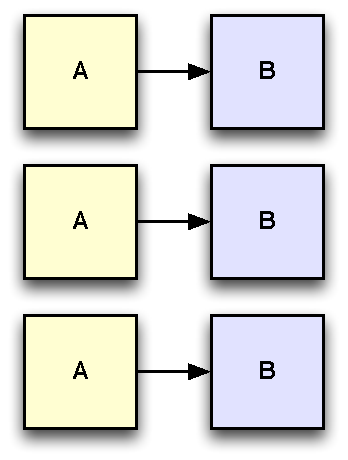
\includegraphics[height=0.43\textheight]{Images/C5/one-to-one.pdf}
    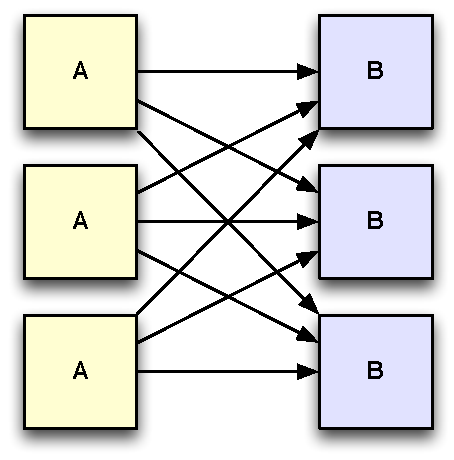
\includegraphics[height=0.43\textheight]{Images/C5/all-to-all.pdf}
  \caption{TODO}
  \label{fig:C4/one-to-one.pdf}
\end{figure}

A `one-to-one' connection is where every $A$ block communicates with exactly one $B$ block, as shown in Figure \ref{fig:C4/one-to-one.pdf}. 
With this type of connection, the number of $A$ blocks must be equal to the number of $B$ blocks.
The F-engines in a FX correlator are a good example of this type of connection. 
The correlator has an F-engine for each antenna, each containing the same blocks linked in the same way. 
Within an F-engine, a PFB\_FIR filter must communicate with a single FFT.
In general, every PFB\_FIR within an F-engine, blocktype `A' must communicate with exactly one FFT, blocktype `B'. 

An `all-to-all' connection occurs when every $A$ block must send some data to ever $B$ block. 
Figure \ref{fig:C4/one-to-one.pdf} shows what an all-to-all connection between three $A$ blocks and three $B$ blocks will look like. 
In this case, every $A$ block must send some data to every $B$ block. 
For example, the type of connection between the per-antenna FFTs and the per-channel X-engines in an FX correlator would be `all-to-all'. 
Each X-engine needs a small amount of data from every F-engine to compute the cross-correlations from a single channel. 
In the `all-to-all' case, there is no reason for the number of sending nodes needs to be the same as the number of receiving nodes. 
%The n's do not get introduced until the ILP is defined
%This means that $n_{i,A}$ and $n_{i,B}$ do not have to be equal, and as long as the data can be distributed appropriately, there is no enforced relationship between the two variables. 




\begin{figure}
  \centering
    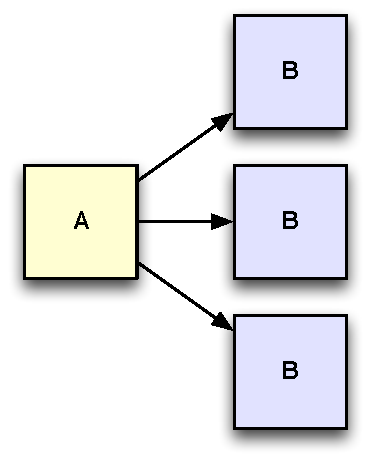
\includegraphics[height=0.45\textheight]{Images/C5/one-to-all.pdf}
    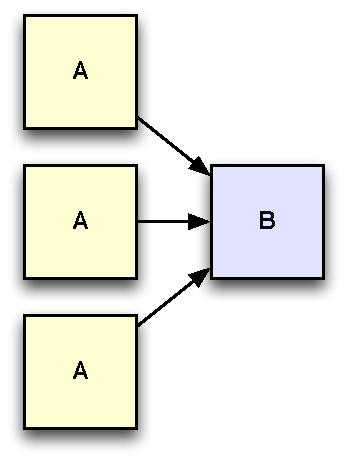
\includegraphics[height=0.45\textheight]{Images/C5/all-to-one.pdf}
  \caption{TODO}
  \label{fig: C4/one-to-all_vs_all-to-one}
\end{figure}



It might seem like there are two more possible types of connection that need to be defined, `one-to-all' and `all-to-one' .
A data flow with a `one-to-all' connection, shown on the left in Figure \ref{fig: C4/one-to-all_vs_all-to-one} would have exactly one $A$ block that needs to send data to many $B$ blocks. 
This is exemplified in the dataflow for a high-resolution spectrometer.
The coarse channelization is done in a single FFT block, which then needs to send the data to many other FFTs to do the fine channelization. 
The `all-to-one' connection is also shown on the right in Figure \ref{fig: C4/one-to-all_vs_all-to-one}
is the reverse of the `one-to-all' case. 
In this type of connection, there are many $A$ blocks and they all need to send data to a single instance of a $B$ block. 
An example of this arises when some processing is done in a distributed manner but the instrument needs to record the final result in a central place. 

It turns out, these are both special instances of the `all-to-all' connection. 
The `one-to-all' connection is simply an `all-to-all' where the number of $A$ blocks is fixed at one.
Similarly, the `all-to-one' connection is also an `all-to-all' where the number of $B$ blocks is fixed at one.
Because of this, there is no need to include or support these cases as unique connection types. 


While it may seem like additional link types exist like `all-to-some' or `one-to-some', this turns out to be impossible. 
Either a block of type $A$ cannot send its data to only some blocks of type $B$ because of the way blocktypes are defined.
Any block of the same type should be interchangeable with another block of the same type.
In an `all-to-some' connection, blocks of type $A$ would need to send data to $B_1$ but not send data to $B_2$.
But that connection patterns implies that the blocks $B_1$ and $B_2$ are \emph{not} interchangeable and therefore cannot have the same blocktype.


%TODO: This isn't implemented in the ILP
%TODO: Add correlator beamformer example. 
%This does not preclude asymmetrical designs. 
%Instead, asymmetry is supported by allowing blocks to define a list of blocktypes they must send data to or receive data from. 
%The connection between any two blocktypes still must be described as above.

%\subsection{Translating Instrument Definitions to Dataflow Diagrams}
% Describe data flow for each instrument we are interested in implementing
%Now that we have a method for describing a general dataflow, we will describe how each type of instrument definition described in the previous section is converted to a dataflow. 
%Multiple antennas?






\section{Mapping}  \label{High Level Toolflow:Mapping}
%TODO: Add tool name
%\begin{figure}[h!]
%  \centering
%    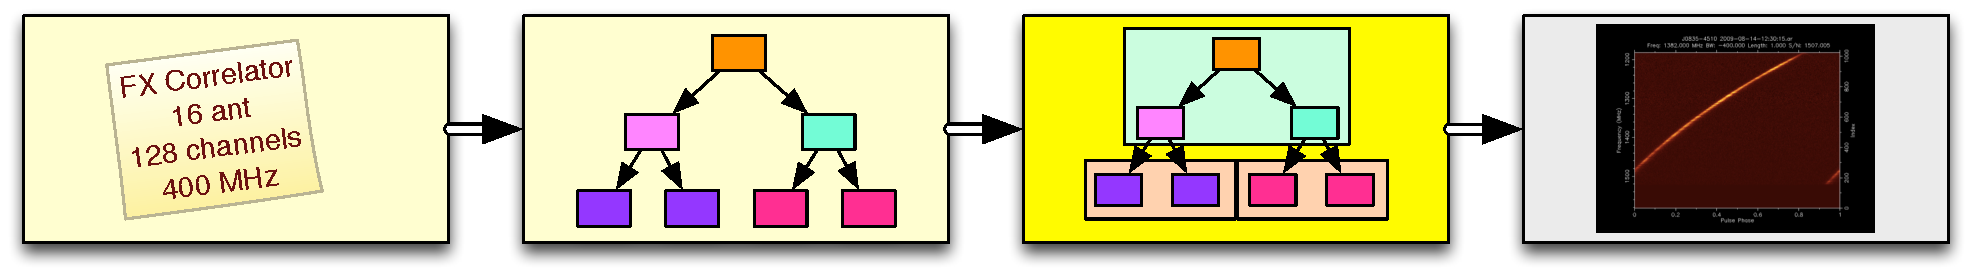
\includegraphics[width=1\textwidth]{Images/C4/toolflow_horizontal_s3.pdf}
%  \caption{ORCAS Toolflow: Mapping}
%  \label{fig: C4/toolflow_horizontal_s3.pdf}
%\end{figure}

\begin{figure}[ht!]
  \centering
    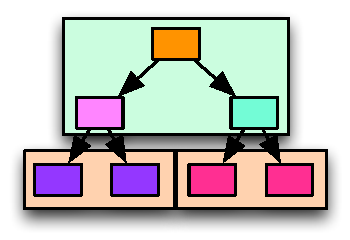
\includegraphics[width=0.75\textwidth]{Images/C4/mapped_dataflow.pdf}
  \caption{The ORCAS Toolflow: Mapped Dataflow Representation}
  \label{fig: C4/mapped_dataflow.pdf}
\end{figure}

Once the dataflow and the computational blocks are defined, ORCAS must determine how to place each computational block into hardware. 
In the mapping stage, ORCAS determines what type of hardware should be used for each block, while minimizing the total cost of the hardware (in dollars, watts, or another used-defined metric).
The icon in Figure \ref{fig: C4/mapped_dataflow.pdf} represents the mapping phase of the toolflow. 

%Not certain this belongs here, possibly should go with the models?
%Before mapping, need to determine which blocks can be mapped to which platforms
%Synthesize/compile existing implementations to determine which platforms can support the spec
%Sanity check bandwidth requirements
%Test for acceptable noise tolerance in different implementations
%Known signals
%Test against arbitrary precision (exact) floating point implementation

At this point, the computational blocks and dataflow can no longer be viewed as abstract algorithms. 
Each computational block must be paired with a performance model for each supported platform that shows the resource utilization and bandwidth requirements for that block. 
Using the performance model, the tool is able to test a number of hardware mappings and ensure that none of the available hardware or bandwidth resources are overmapped.

The optimal mapping is determined using an Integer Linear Program or ILP. 
The resources, such as memory, logic and CPU time, and bandwidth constraints are translated directly into ILP constraints.
These constraints are used to determine a valid mapping, for example total bandwidth mapped to a link must be less than total link bandwidth.
The variables represent the design decisions, determining where each block should be implemented.
And finally, the cost function simply totals up the costs associated with each piece of hardware used.

%TODO: rewrite with references
A ILP was chosen because it has a number of positive features.
Unlike a randomized algorithm such as simulated annealing, the results from a ILP are repeatable.
While there might be multiple solutions with the same cost, each time the same ILP is run, it is guaranteed to find one of the solutions of optimal cost. 
The ILP representation also makes it easy for the user to guide the algorithm. 
Since the design choices are represented by variables, they can also be restricted by adding additional constraints to those variables.
This representation also makes it easy to build out an existing cluster, by allowing a limited amount of zero-cost hardware.

Unfortunately, the advantages of the ILP come with a high cost, namely that an ILP is NP-Hard to solve optimally.
%TODO: ref
Current ILP benchmarks are able to solve problems with a hundred thousand variables in a few hours, but beyond that size the problems become infeasible.
%TODO: add an ex solver
To make matters worse, the ILP runtime is very sensitive to the solver being used and the problem structure.

Because the runtime for the ORCAS mapper needs to be within a few hours, we use a number of techniques to reduce the ILP runtime.
%TODO: add more info here
First, the easiest way to reduce the runtime without changing the ILP is to change the solver. 
There is a huge amount of variance in runtimes between different solvers and simply switching out the backend solver might cause a previously infeasible problem to become solvable.
When that doesn't improve the runtime enough, it becomes necessary to modify the ILP.
One way to do this is by reducing the number of variables it needs to solve for.
Many of the radio astronomy instruments are very symmetric, so it is reasonable to assume that the optimal mapping would be symmetric as well.
The symmetry can be preserved by forcing every block of a certain type to be implemented in the same kind of hardware, drastically reducing the number of decisions that the ILP needs to make.
The ILP can also be modified to ensure that there is a single, unique optimal solution.
When designs are very symmetric, the ILP will often find an optimal solution quickly but, because it is not unique, the ILP must spend a lot of time convincing itself that the solution is, in fact, optimal.
Additional constraints can be added to ensure that only one of those solutions is valid, greatly reducing the amount of time it takes to verify optimality.

Chapter \ref{chap:Algorithm Partitioning} goes into more detail on how the performance models are used as well as how the ILP is specified and optimized to achieve a feasible runtime. 

\subsection{Mapped Dataflow Representation}

\begin{figure}[ht!]
  \centering
    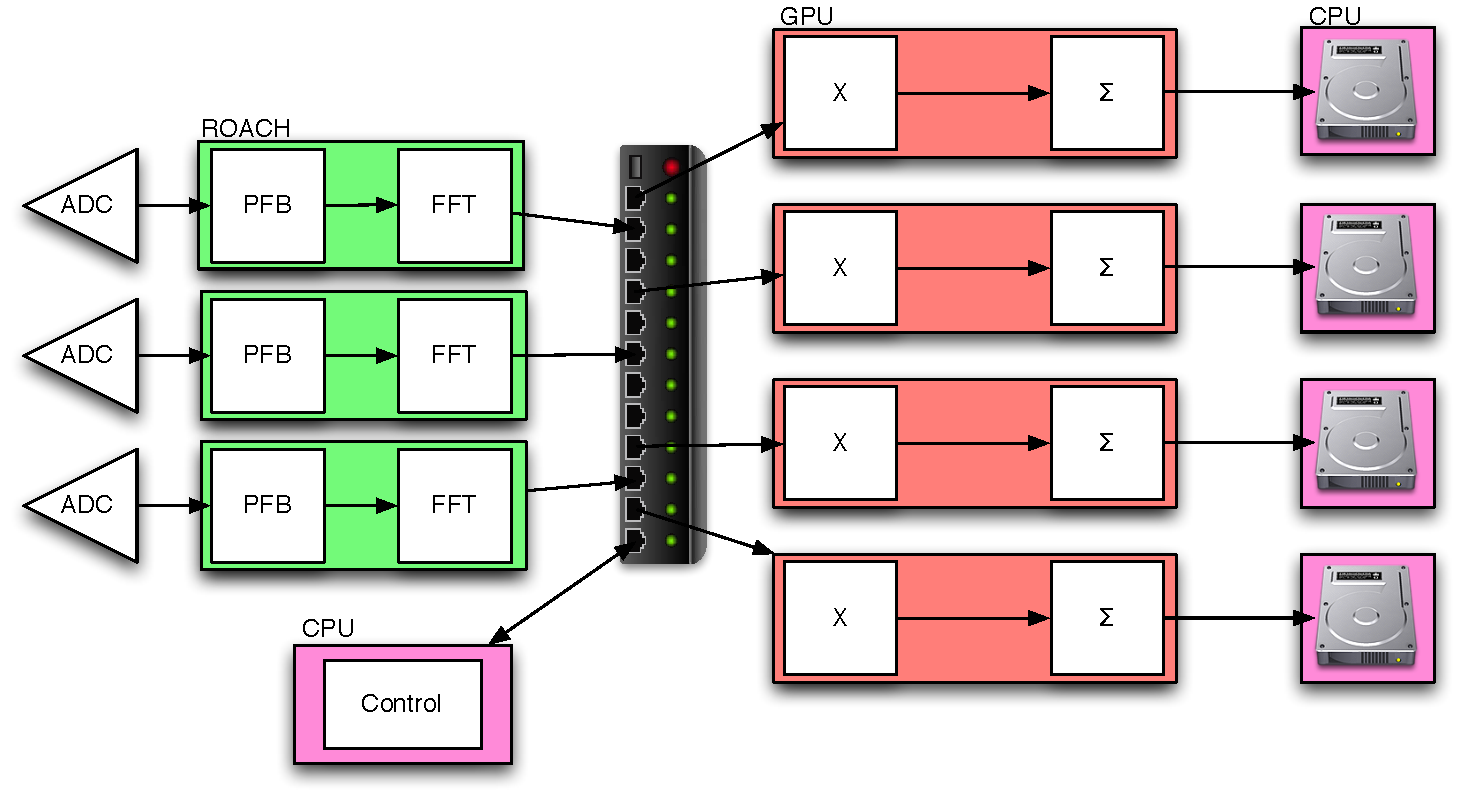
\includegraphics[width=\textwidth]{Images/C4/fx_mapped.pdf}
    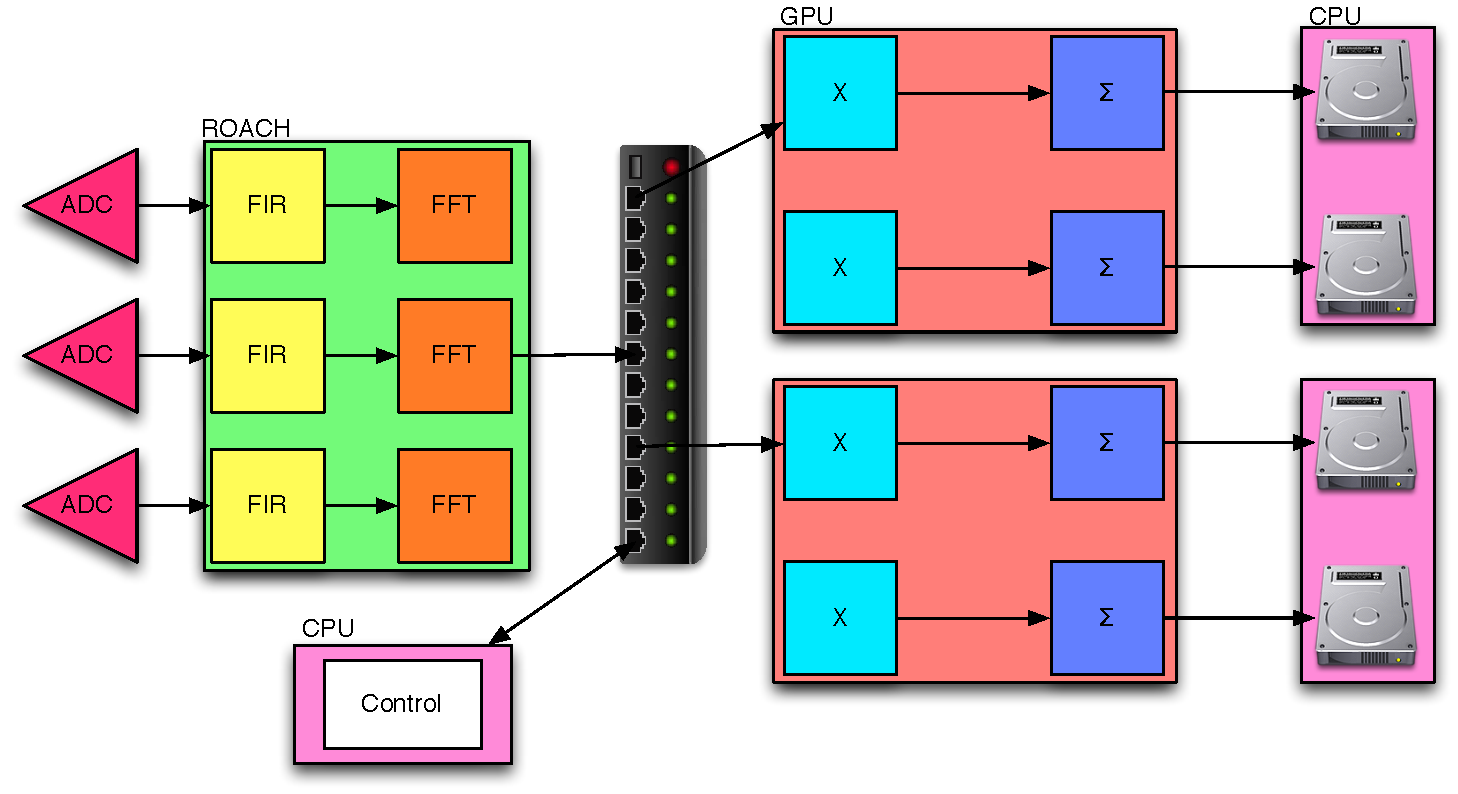
\includegraphics[width=\textwidth]{Images/C4/fx_mapped_alt.pdf}
  \caption{Two potential mappings for the FX Correlator}
  \label{fig: C4/fx_mapped.pdf}
\end{figure}

Once the mapping is complete, the dataflow model is updated to describe what type of hardware will be used to implement each computational block.
Figure \ref{fig: C4/fx_mapped.pdf} shows two or many possible mappings for the FX Correlator dataflow shown in Figure \ref{fig: C4/fx_dataflow.pdf}.
In the top dataflow, each F-engine and X-engine require so many resources that they must be implemented on separate boards.
Each F-engines is implemented on an FPGA-based ROACH board and the X-engines are implemented in GPUs.
The bottom dataflow shows a less resource-hungry correlator, allowing all the F-engines and two X-engines to share a single board for computation.

In all designs, any link between two blocks that are not mapped to the same board must pass through a switch. 
In the example, all the links between FFTs and cross-correlation blocks must run through the switch.
This is represented in the diagram by a single connection from each ROACH and GPU board to the switch.


\section{Code Generation} \label{High Level Toolflow:Code Generation}
The last step in the process is the implementation the instrument. 
This step is optional, only being used when the mapped dataflow is being used to design an instrument rather than assess cost. 
Since the toolflow relies on established libraries, implementation only consists of stitching together existing routines.

%\begin{figure}[ht!]
%  \centering
%    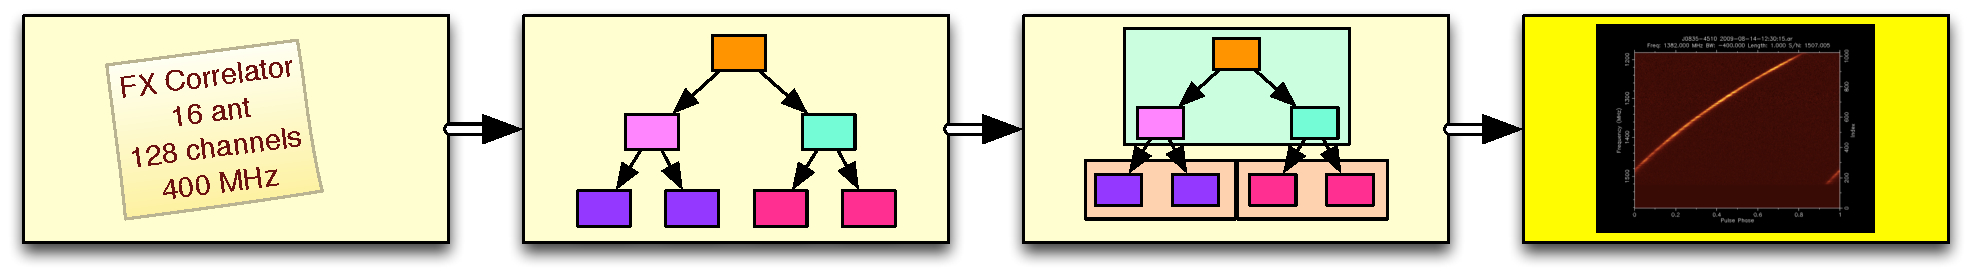
\includegraphics[width=1\textwidth]{Images/C4/toolflow_horizontal_s4.pdf}
%  \caption{The ORCAS Toolflow: Code Generation}
%  \label{fig: C4/toolflow_horizontal_s4.pdf}
%\end{figure}


In addition to this, common design patterns can be stitched together into parameterized implementations. 
This style of instrument design greatly accelerates time to science for many projects.
Separating the implementation of the instrument from the hardware specification has created a design that works well for a variety of computational resources and applications.
As resources improve, the instrument can improve along with them, providing the opportunity to do new science that wasn't possible on older technology.
We have shown this is possible by implementing the Packetized Astronomy Signal Processor or PASP using the CASPER toolflow. \cite{Filiba:2011wl}









 
\chapter{Algorithm Partitioning}

%Summary: add on the idea of the partitioner to reconfigurable instrumentation rather than the partitioning coming from a person we can use a computer to optimize this
%describe linear program in detail
%describe and defend design choices/heuristics/approximations
%Goal: show how to do cost-driven partitioning of a design
%for now �cost� and �performance� are still variables
%State: intro to ILP can be written now. documenting the actual ILP for this application will be done after the analysis/results

\section{Constraints}

\section{Cost}

\section{Optimization}


\section{Performance}
%TODO: this will have to be written after ch 6 is complete, to make sure we are benchmarking the correct thing. in the meantime we'll write in introduction  
\chapter{Analysis} \label{chap:Analysis}

%TODO: edit this awkwardness
The ORCAS tool is analyzed by looking at three case studies. 
We created three instrument types: Spectrometer, High Resolution Spectrometer, and FX Correlator, as defined in Sections \ref{Real Time Radio Astronomy Algorithms:Spectroscopy}, \ref{Real Time Radio Astronomy Algorithms:Pulsar Processing}, and \ref{Real Time Radio Astronomy Algorithms:Correlation}. 
Each case study was chosen to illustrate a different aspect of the toolflow.
The spectrometer gives an example of the end to end toolflow using a simple dataflow, the high resolution spectrometer allows us to explore tradeoffs in the design space and the FX correlator shows how the tool behaves when designing very large instruments.


%Simple spectrometer placement

%TODO: Include appropriate FFT or PFB benchmarks

%Summary: describe how we get real numbers to put into previous part
%Goal: define and obtain real numbers from the previous part
%\section{Benchmarks}

%\subsection{Cost}

%Summary: case studies describing partitioning of realistic-scale instruments
%Goal: show successful application of tool to design of realistic instruments
%provide analysis comparing this to hand-designed instruments 
\section{Spectrometer Case Study}
The spectrometer is a simple instrument, making it easy to follow the end to end toolflow.
We design %a 50 MHz and 
an 800 MHz spectrometer that breaks the band into 1024 channels.
%TODO: what is a reasonable integration time here


\subsection{Spectrometer Definition}
Defining a simple spectrometer requires very few parameters. 
First, as with most instruments, the astronomer must specify the sky bandwidth the instrument must process, defined in MHz and the number of bits in each ADC sample.
Then, the desired spectral resolution is defined in MHz per channel, or analogously, the number of channels that should be used to break up the bandwidth.
Finally, the integration time needs to be defined.

One optional parameter, number of antennas, can also be defined. 
This describes the number of independent spectrometers that need to be created.
While this parameter does not affect the end to end processing for each antenna, knowing how many spectrometers are needed allows for more efficient use of the hardware.

The 800 MHz spectrometer is created simply by defining the parameters and instantiating a Spectrometer object as follows:

\lstinputlisting[language=Python,
    %caption=My Class,
    label={spec_defn.py},
    breaklines=true,
  ]{code/C6/spec_defn.py}

\subsection{Spectrometer Dataflow}

%TODO: add detection step
\begin{figure}[ht!]
  \centering
    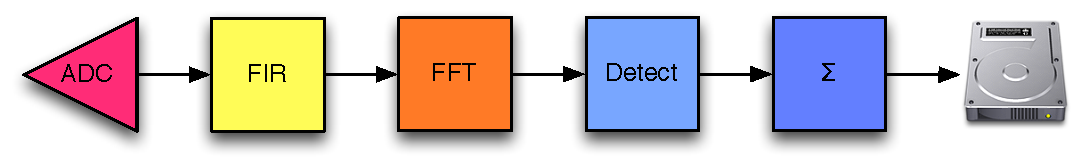
\includegraphics[width=1\textwidth]{Images/C4/spectrometer_dataflow.pdf}
  \caption{General Spectrometer Dataflow Model}
  \label{fig: C4/spectrometer_dataflow.pdf}
\end{figure}

The spectrometer instrument definition generates a very simple dataflow. 
Figure \ref{fig: C4/spectrometer_dataflow.pdf} shows the general dataflow model for a single antenna spectrometer. 
This model can be applied to any spectrometer, as the spectrometer parameters do not affect how many computational blocks are required or the interconnect layout. 
The ADC feeds data into a FIR filter. 
Then the filtered signal is transformed into channels in the FFT and those channels are accumulated and saved to disk. Regardless of the parameters the astronomer chooses, the dataflow will be the same. 

The parameters for each block come directly from the instrument definition. 
The FIR parameters come from the number of FIR taps and window shape, the FFT is simply defined by the FFT length parameter and the accumulator also is parameterized by the FFT length as well as the integration time. 
The code below shows how the blocks are added to the dataflow model.

\lstinputlisting[language=Python,
    %caption=My Class,
    label={spec_dflow.py},
    breaklines=true,
  ]{code/C6/spec_dflow.py}

\subsection{Spectrometer Mapping}
As a simple case study, an 1024 channel 800 MHz spectrometer is mapped using the ROACH and GTX 580-based NRAO server as potential platforms. 
ORCAS produces a solution that maps the entire design to a single ROACH board.
This solution is obviously correct since the bandwidth cannot be processed by a single GPU and a single ROACH is cheaper than a combination of boards.
The mapping produced by ORCAS is shown below.

\lstinputlisting[
    %caption=My Class,
    label={spec_dflow.py},
    breaklines=true,
  ]{code/C6/spec_800_result.txt}
  

%\lstinputlisting[
%    %caption=My Class,
%    label={spec_dflow.py},
%    breaklines=true,
%  ]{code/C6/spec_050_result.txt}
  
%\subsection{Cost}
%\subsection{Power}

\section{High Resolution Spectrometer Case Study}
The high resolution spectrometer is a useful instrument for SETI. 
The two stage channelization creates a large number of channels without using an FFT that is too large to fit on a single board.


\subsection{High Resolution Spectrometer Definition}
The main difference between a spectrometer and a high resolution spectrometer is the need for two stages of channelization rather than just one. 
The sky bandwidth, integration time, and number of antennas are defined in the same way as the previous spectrometer type. 

The spectral resolution is defined differently, because both the coarse and fine resolutions need to be defined. 
The coarse resolution defines how many channels the whole sky bandwidth should be broken up into initially.
The fine resolution defines how many channels each coarse channel is broken into.
Both can be described in MHz per channel.

\subsection{High Resolution Spectrometer Dataflow}

%TODO: add detection step
\begin{figure}[ht!]
  \centering
    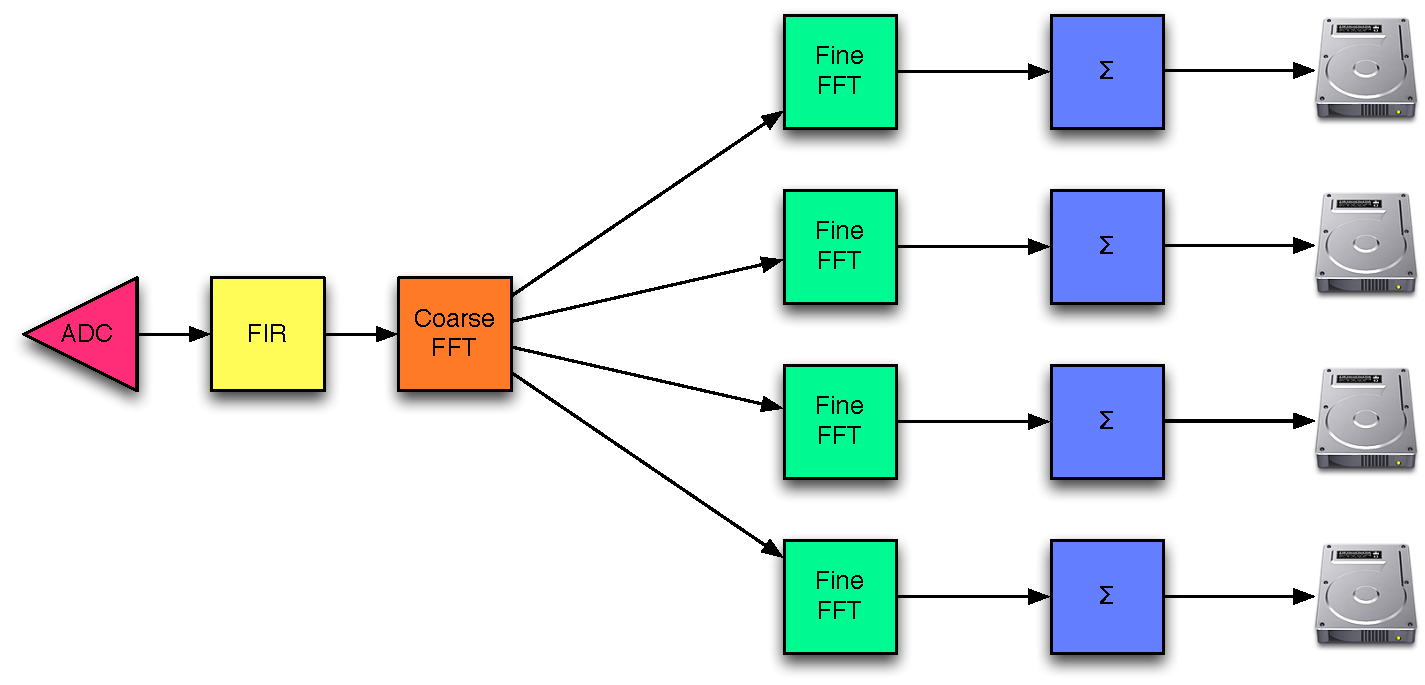
\includegraphics[width=1\textwidth]{Images/C4/hires_spectrometer_dataflow.pdf}
  \caption[Example High Resolution Spectrometer Dataflow Model]{Example High Resolution Spectrometer Dataflow Model
  \textit{
  This figure shows an example dataflow for a high resolution spectrometer with 4 coarse FFT channels.
  Like the previous spectrometer, the data comes in through an ADC, is filtered and then channelized using a coarse FFT.
  Then, to achieve a higher resolution, each coarse channel is divided into sub-channels using the 4 fine FFT blocks in the dataflow. 
  }}

  \label{fig: C4/hires_spectrometer_dataflow.pdf}
\end{figure}

The high resolution spectrometer dataflow does depend on the parameters specified in the instrument description. 
An example dataflow is shown in Figure \ref{fig: C4/hires_spectrometer_dataflow.pdf}. 
The first three blocks in the dataflow are exactly the same as the Spectrometer dataflow described in the previous section. 
An ADC feeds data into a FIR filter followed by an FFT. 
After the FFT, the algorithm is modified to accommodate the higher resolution required. 
The first FFT divides the band into a number of coarse channels and then each coarse channel must be further divided into a number of fine channels. 
The coarse FFT must feed its data to a separate fine FFT for each coarse channel, so the number of fine FFTs in the dataflow diagram will vary based on the number of coarse channels.
At this point, each coarse channel is processed in an independent pipeline the finely channelized data is accumulated and recorded to disk. 
The example in Figure \ref{fig: C4/hires_spectrometer_dataflow.pdf} shows a spectrometer that divides the data into 4 coarse channels.

%\subsection{Cost}
%\subsection{Power}

\subsection{Algorithmic Exploration}

The Arecibo L-band feed array, pictured in Figure \ref{fig: C3/alfa_feed.png} has 7 dual-polarization beams. 
The SERENDIP V.v instrument was only able to process one beam at a time, but its planned successor, SERENDIP 6, will process 300MHz from each beam-pol.

\begin{figure}[ht!]
  \centering
    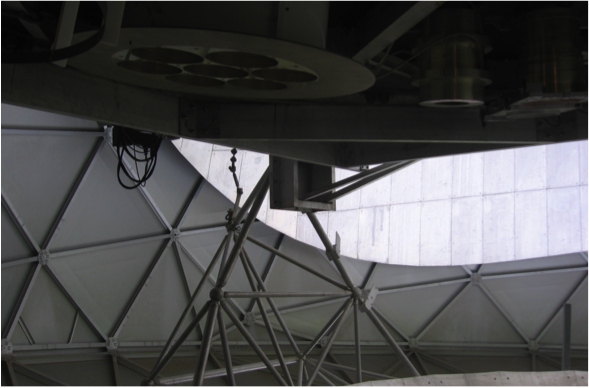
\includegraphics[width=\textwidth]{Images/C3/alfa_feed.png}
  \caption{Arecibo ALFA Feed}
  \label{fig: C3/alfa_feed.png}
\end{figure}

In this case study, we analyze the design space for a 300 MHz 256 million channel spectrometer, similar to the SERENDIP 6 instrument.
This instrument provides an interesting case study because the number of channels is so large.
The number of channels in the coarse and fine FFTs can be varied, as long as the product remains 256 million.
We explore this design space by varying the dimensions and number of antennas to see how the channel balance affects the final cost of the instrument.

This instrument is designed using ROACH boards and the GTX 580-based NRAO server as supported platforms, and uses the FIR and FFT benchmarks presented in Chapter \ref{chap:Algorithm Partitioning}
To aid the linear program, we assume reordering the coarse FFT data is infeasible on the GPU and force the design to reorder the data on the FPGA.


\begin{sidewaystable}
\begin{tabular}{| c | c | c | c | c | c |}
\hline  
\diaghead{\theadfont Diag ColumnmnHead II}{\textbf{Antennas}}{\textbf{Dimensions}} & 256 by 524,288 & 512 by 262,144 & 1024 by 131,072 & 
2048 by 65,536 & 4096 by 32,768\\
\hline  
1 &  \begin{tabular}{c} 2 GPUs \\ 1 ROACH \\ \$13.7k \end{tabular} & \begin{tabular}{c} 2 GPUs \\ 1 ROACH \\ \$13.7k \end{tabular} & \begin{tabular}{c} 2 GPUs \\ 1 ROACH \\ \$13.7k \end{tabular} & \begin{tabular}{c} 1 GPU \\ 1 ROACH \\ \$10.2k \end{tabular} &\begin{tabular}{c} 1 GPU \\ 1 ROACH \\ \$10.2k \end{tabular}  \\
\hline
3  & \begin{tabular}{c} 5 GPUs \\ 1 ROACH \\ \$24.2k \end{tabular} & \begin{tabular}{c} 4 GPUs \\ 1 ROACH \\ \$20.7k \end{tabular} & \begin{tabular}{c} 4 GPUs \\ 1 ROACH \\ \$20.7k \end{tabular} & \begin{tabular}{c} 3 GPUs \\ 1 ROACH \\ \$17.2k \end{tabular} & \begin{tabular}{c} 3 GPUs \\ 2 ROACH \\ \$23.9k \end{tabular} \\
\hline  
5 & \begin{tabular}{c} 8 GPUs \\ 2 ROACH \\ \$41.4k \end{tabular} & \begin{tabular}{c} 7 GPUs \\ 2 ROACH \\ \$37.9k \end{tabular} & \begin{tabular}{c} 7 GPUs \\ 2 ROACH \\ \$37.9k \end{tabular} &
 \begin{tabular}{c} 5 GPUs \\ 2 ROACH \\ \$30.9k \end{tabular} &  \begin{tabular}{c} 5 GPUs \\ 2 ROACH \\ \$30.9k \end{tabular} \\
\hline  
7 & \begin{tabular}{c} 12 GPUs \\ 2 ROACH \\ \$55.4k \end{tabular} & Not solved & \begin{tabular}{c} 9 GPUs \\ 3 ROACH \\ \$51.6k \end{tabular}  &
 \begin{tabular}{c} 8 GPUs \\ 3 ROACH \\ \$48.1k \end{tabular} &  \begin{tabular}{c} 7 GPUs \\ 3 ROACH \\ \$44.6k \end{tabular}\\
\hline  
\end{tabular}
\caption{134 Million Channel High Resolution Spectrometer Design Space}
\label{tab: C5/highres_spec_design_space}
\end{sidewaystable} 

Table \ref{tab: C5/highres_spec_design_space} shows the results of this design space exploration. 
We observe that extreme values for the number of channels tends to increase costs, likely because it's difficult to put larger blocks together on the same board and get high utilization of the hardware.
Each test was run with a 30 minute time limit on my personal laptop, a 2011 Macbook Air, to ensure that the designs could converge quickly.
One test, the 7 antenna 512 by 262,144 channel spectrometer did not converge within the specified time.
While it might be able to converge given more time, the resulting table make it clear that the optimal configuration is unlikely to lie in that square, and there is no need to spend extra time trying to get a solution.

%results for hi res spectrometer (gbt and seti)

%Serendip 6 300MHz 7 ant 2 pol

%1Hz resolution (256 million channels)

%Greenbank 2.5GHz 1 beam 2 pols

%1 Hz resolution

%Same benchmarks as before, just discuss large bw, multi stage fft



\section{FX Correlator Case Study}
\subsection{FX Correlator Definition}
An FX Correlator is also defined by the amount of bandwidth it processes, number of channels, and integration time, but now the number of antennas is a necessary parameter.

\subsection{FX Correlator Dataflow}

The FX dataflow model is based on the algorithm used by the CASPER correlator described in Section \ref{Related Work:Radio Astronomy}. The processing model is described by replicating 2 basic pipelines, called an F-Engine and an X-Engine. The number of times each pipeline needs to be replicated depends on the number of antennas and number of channels this correlator requires.

\begin{figure}[h!]
  \centering
    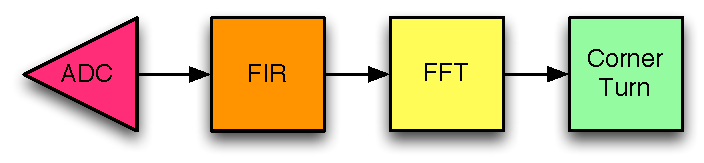
\includegraphics[width=0.48\textwidth]{Images/C4/fx_f_engine.pdf}
  \caption{FX Correlator F-Engine Model}
  \label{fig: C4/fx_f_engine.pdf}
\end{figure}

An F-Engine, pictured in Figure \ref{fig: C4/fx_f_engine.pdf} is responsible for channelizing the data from a single antenna. 
%TODO: explain or reference PFB (should be explained in C2 or 3?)
It takes in data from an ADC, and channelizes the data using a FIR and FFT to create a polyphase filter bank. 
The number of F-Engines in the correlator dataflow will vary with the number of antennas.

%TODO: add detection step
\begin{figure}[h!]
  \centering
    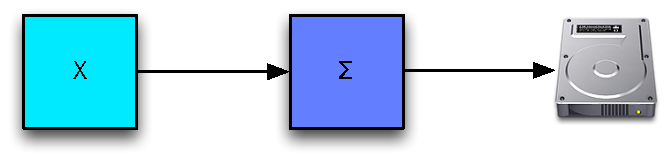
\includegraphics[width=0.48\textwidth]{Images/C4/fx_x_engine.pdf}
  \caption{FX Correlator X-Engine Model}
  \label{fig: C4/fx_x_engine.pdf}
\end{figure}

The second pipeline, the X-Engine processes the channelized data. 
Each X-Engine takes a single channel of data from every antenna in the array, cross-correlates the data, accumulates it and stores it to disk. 
Figure \ref{fig: C4/fx_x_engine.pdf} shows the pipeline for a single X-Engine. 
Since each X-Engine only operates on a single channel, the total number of X-Engines in the correlator must be the same as the number of channels in the FFT.

%TODO: add detection step
\begin{figure}[h!]
  \centering
    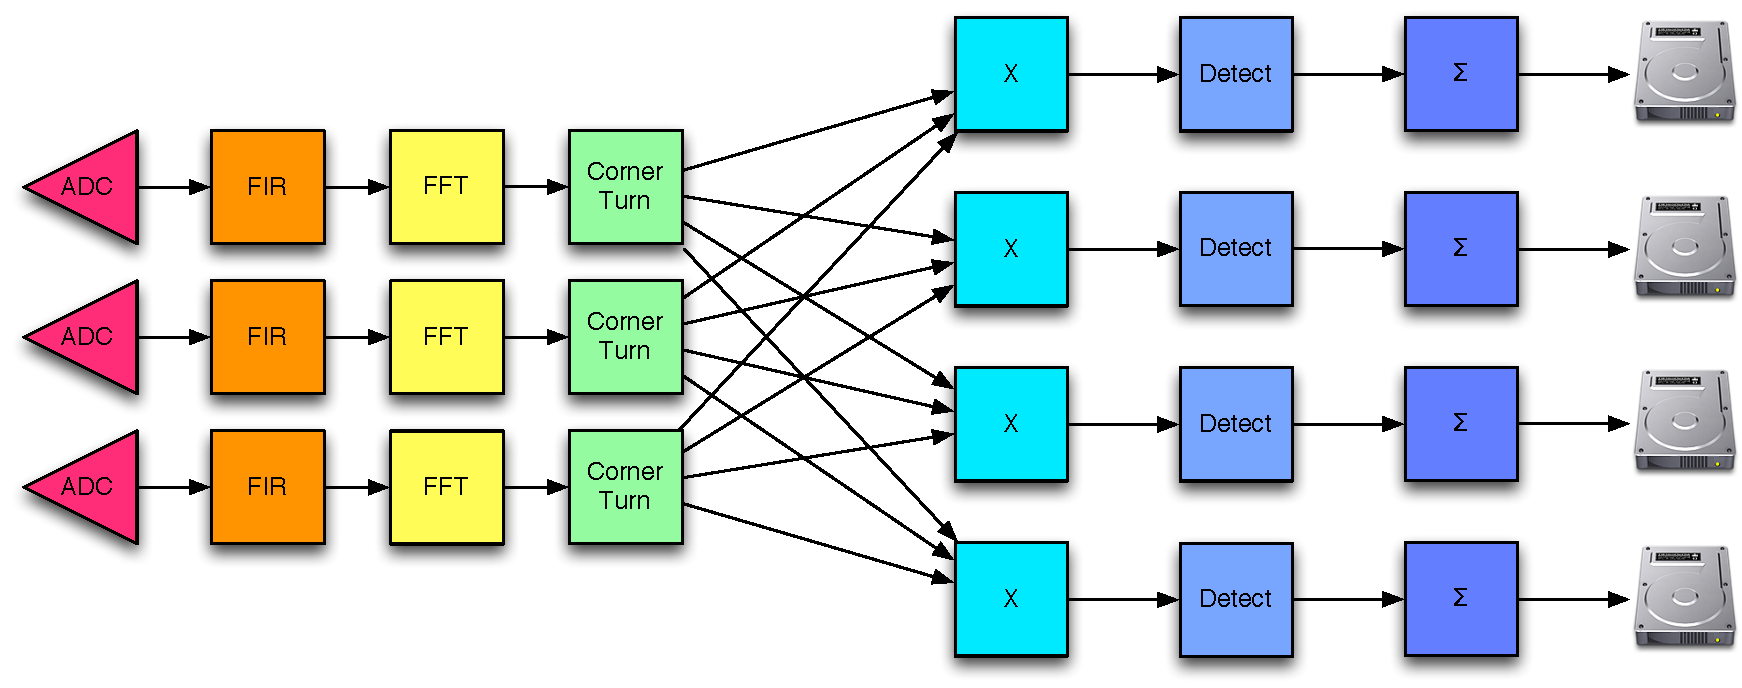
\includegraphics[width=1\textwidth]{Images/C4/fx_dataflow.pdf}
  \caption{Example FX Correlator Dataflow Model}
  \label{fig: C4/fx_dataflow.pdf}
\end{figure}

The dataflow for an FX correlator will vary quite a bit based on the input parameters. 
Figure \ref{fig: C4/fx_dataflow.pdf} shows an example there antenna four channel FX correlator. 
The left half of the figure has three F-engines, for each of the three antennas.
The right half has four X-engines, one for each channel.
And in the center, since each X-engine requires data from every F-engine, the cross-correlation blocks, represented by an \emph{X} and the FFT blocks are connected in an all-to-all configuration.

\subsection{FX Correlator Mapping}
The FX Correlator is evaluated by investigating at how correlator design scales from 16 to 572 antennas.
%TODO: remove

\emph{Note: The benchmarks are still being refined. An updated version of the results will be available on Monday}

The 572 antenna design is based on the planned HERA Correlator.
This correlator processes 100 MHz of data and divides it into 1024 channels.


 
\chapter{Conclusions}
\label{chap:Conclusions}

%Summary: summarize work and impact, describe directions for further work, describe how this provides a framework for an end to end solution in radio astronomy as well as other domain specific applications
%Goal: show everything worked and was awesome
%State: needs results, should be quick to write but difficult to write now

%TODO: explain this in text
This dissertation presents an end to end solution that allows domain experts to take a high level idea and and translate it into a design indicating what types of hardware should be used to implement the instrument. 
The ORCAS tool is able to generate these designs quickly, making it a useful tool to explore the design space of different astronomy algorithms.
I demonstrate three types of instrument design, and explore how changing the parameters affects the implementation and costs of these instruments.



\section{Future Work}
The success of this work opens up a lot of related projects to improve upon the existing mapping capabilities.
While the instruments developed with ORCAS are designed for radio astronomy, ORCAS was developed as a general purpose tool and the expansion of the instrument set into other fields would provide interesting new challenges.
The existence of a DSP library and benchmarks would make it easy to transition to other DSP applications.

%Design interconenct
Since other applications might not need a full-crossbar network, it would also be useful to integrate network design into the ILP.
In radio astronomy, it is reasonable to assume this network exists and ignore the cost when designing instruments.
The toolflow currently allows the user to minimize the number of ports required but this still assumes the presence of a full-crossbar interconnect.
In applications with different network architectures, the costs can significantly change with the network design as well as the platforms used; future versions of this tool that are used for these applications will need to take those costs into account.


There are also improvements that can be made to the model, but they need to be balanced with the ILP to ensure fast runtimes.
As telescope arrays get larger, a single computational block may need to span multiple boards.
As we saw in the FX Correlator case study, this is going to be the case for the X-Engine in the near future.
Simply supporting that capability would be useful, but it would be better if the model was able to determine how to split these blocks between boards.

%Do a better job of preserving symmetry
Finally, the ILP aims to reduce cost in any way possible and often does so by cramming unrelated blocks onto the same platform.
ORCAS does support an option that forces the tool to create exactly one design on each platform, but this does not prevent the tool from putting unrelated blocks in the same design.
To make the resulting designs more straightforward, it would be useful if the ILP could preserve the problem structure when translating the design to hardware.


%\section{Final Conclusions}
%This work is a major step towards a universal clustered radio astronomy architecture.
%Figure \ref{fig: C5/universal_arch.png} gives an example of what this type of architecture could look like.
%
%
%\begin{figure}[ht!]
%  \centering
%    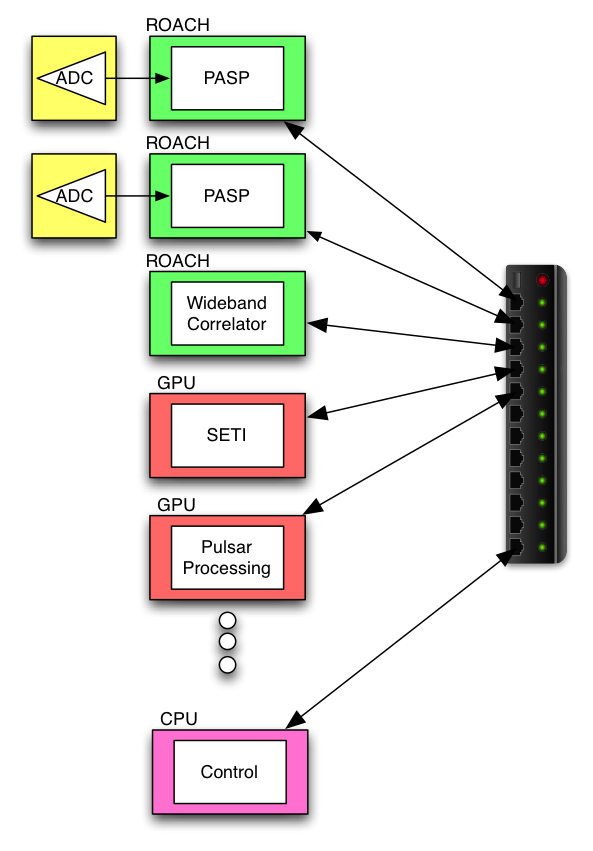
\includegraphics[width=0.5\textwidth]{Images/C5/universal_arch.png}
%  \caption{A potential architecture for multiple scientific instruments simultaneously processing data from the same telescope}
%  \label{fig: C5/universal_arch.png}
%\end{figure}
 


% \appendix
% \chapter{More Monticello Candidates}

\printbibliography

\end{document}
